% !TeX root = ../proyecto.tex

\chapter{Entorno Experimental}\label{ch:entorno-experimental}
En este capítulo se describe el entorno experimental empleado para evaluar los algoritmos propuestos.
Se detallan los conjuntos de datos utilizados, el diseño de los experimentos, el procedimiento de ejecución y las métricas de evaluación.
Asimismo, se explica cómo se presentan y visualizan los resultados obtenidos.


\section{Datasets utilizados}\label{sec:datasets}
En el aprendizaje profundo, los datasets son colecciones de datos etiquetados o no etiquetados que se utilizan para
entrenar modelos.
Estos conjuntos de datos contienen ejemplos organizados que representan la entrada para el modelo y, en muchos casos,
también las etiquetas correspondientes que indican la salida deseada.
Los datasets varían en tamaño, calidad y tipo, dependiendo de la tarea a resolver, como la clasificación de imágenes,
el reconocimiento de patrones o la predicción de series temporales.


A continuación, se van a explicar cada uno de los Datasets que se han utilizado en el desarrollo del proyecto.

\subsection{Rock, Paper, Scissors (Piedra, Papel, Tijera)}\label{subsec:rock-paper-scissors}
\textbf{Rock, Paper, Scissors}~\cite{RockPaperScissors} es un conjunto de datos creado por Laurence Moroney
que se utiliza para la clasificación de imágenes de manos representando los gestos de `piedra', `papel' y `tijeras'.

\begin{figure}[htp]
    \centering
    \begin{subfigure}[t]{0.3\textwidth}
        \centering
        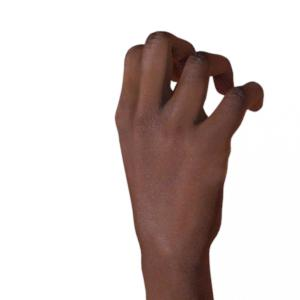
\includegraphics[width=\linewidth]{imagenes/dataset_examples/rock.jpg}
        \caption*{Rock}
    \end{subfigure}
    \begin{subfigure}[t]{0.3\textwidth}
        \centering
        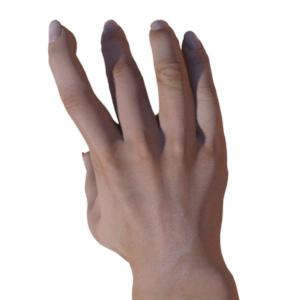
\includegraphics[width=\linewidth]{imagenes/dataset_examples/paper.jpg}
        \caption*{Paper}
    \end{subfigure}
    \begin{subfigure}[t]{0.3\textwidth}
        \centering
        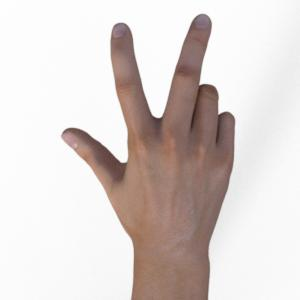
\includegraphics[width=\linewidth]{imagenes/dataset_examples/scissors.jpg}
        \caption*{Scissors}
    \end{subfigure}
    \caption{Ejemplos de imágenes del dataset Rock, Paper, Scissors}
    \label{fig:ejemplos-rps}
\end{figure}

En la figura~\ref{fig:ejemplos-rps} se han mostrado una imagen de cada una de las clases del dataset Rock, Paper, Scissors,
para que se pueda observar la similitud entre las distintas clases.

\subsubsection{Estructura del Dataset}
El conjunto de datos usado contiene 2,925 imágenes, distribuidas en tres categorías: piedra, papel y tijeras.
Las imágenes están en color y tienen un tamaño de 300x300 píxeles.

\begin{figure}[ht]
    \centering
    \begin{forest}mydirstyle
        [RPS
            [train
                    [rock
                            [image1.jpg]
                            [image2.jpg]
                            [\dots]
                    ]
                    [paper
                            [image1.jpg]
                            [image2.jpg]
                            [\dots]
                    ]
                    [scissors
                            [image1.jpg]
                            [image2.jpg]
                            [\dots]
                    ]
            ]
            [test (originalmente valid)
                [rock]
                    [paper]
                    [scissors]
            ]
            [valid (originalmente test)
                [rock]
                    [paper]
                    [scissors]
            ]
        ]
    \end{forest}
    \caption{Estructura de carpetas del dataset Rock, Paper, Scissors}
    \label{fig:estructura-rps}
\end{figure}


Como se puede observar en la Figura~\ref{fig:estructura-rps}, las imágenes están organizadas en directorios según su función en el entrenamiento
(entrenamiento, validación o prueba) y, dentro de cada partición, se dividen a su vez por clases del dataset.

\subsubsection{Formato de los Datos}
Las imágenes están en formato JPEG (\texttt{.jpg}).
Para su procesamiento, se han aplicado técnicas de preprocesamiento
adaptadas a los requerimientos del modelo.

\subsubsection{Uso del Dataset}
Este dataset se ha utilizado para evaluar el rendimiento del modelo en un problema de clasificación de imágenes con
múltiples clases, pero siendo un dataset sencillo y con un número de clases pequeño.
Además, permite explorar la eficacia de los algoritmos meméticos en un entorno más cercano al reconocimiento de objetos.

\subsubsection{Correcciones en la División de Datos}
Según la nota observada en el README del dataset:
\begin{quote}
    \textit{Note: in the source, Laurence calls ``validation'' as the ``test'', and ``test'' the ``validation''.}
\end{quote}
se han renombrado las particiones de \texttt{test} y \texttt{valid} para que correspondan correctamente con sus
propósitos.

\subsubsection{Licencia y uso}
Este conjunto de datos se distribuye bajo la licencia
\textbf{Creative Commons Attribution 4.0 International (CC BY 4.0)}, lo que permite su uso, modificación y distribución
con la condición de otorgar el crédito adecuado a los creadores originales.


\subsection{PAINTING (Art Images: Drawing/Painting/Sculptures/Engravings)}\label{subsec:painting}
El dataset \textbf{Art Images: Drawing/Painting/Sculptures/Engravings} usado es una colección de 8.576
imágenes organizadas en cinco categorías de arte: dibujos, pinturas, esculturas, grabados y arte iconográfico.

\begin{figure}[htp]
    \centering
    \begin{subfigure}[t]{0.3\textwidth}
        \centering
        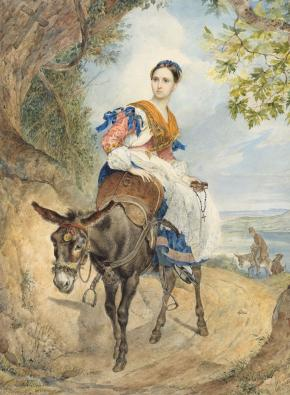
\includegraphics[width=\linewidth]{imagenes/dataset_examples/drawings.jpg}
        \caption*{Drawings}
    \end{subfigure}
    \begin{subfigure}[t]{0.3\textwidth}
        \centering
        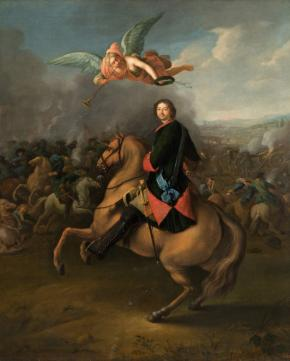
\includegraphics[width=\linewidth]{imagenes/dataset_examples/painting.jpg}
        \caption*{Painting}
    \end{subfigure}
    \begin{subfigure}[t]{0.3\textwidth}
        \centering
        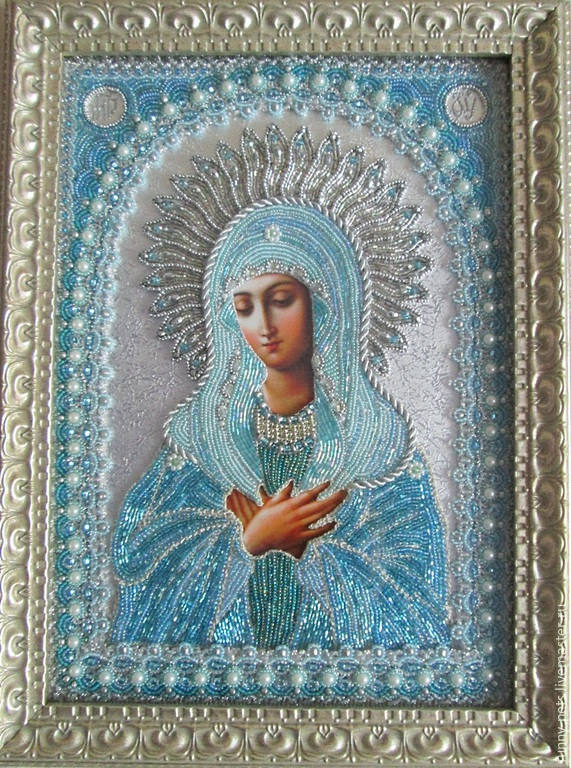
\includegraphics[width=\linewidth]{imagenes/dataset_examples/iconography.jpg}
        \caption*{Iconography}
    \end{subfigure}
    \begin{subfigure}[t]{0.3\textwidth}
        \centering
        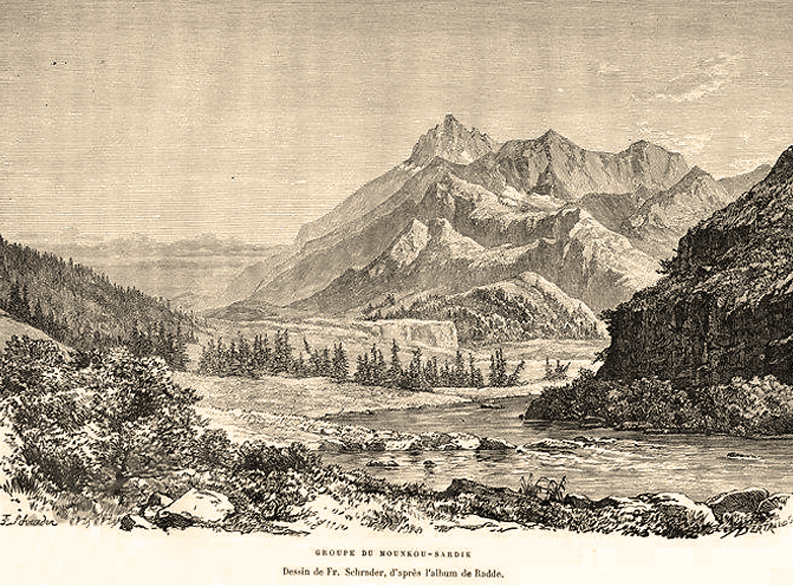
\includegraphics[width=\linewidth]{imagenes/dataset_examples/engraving.jpg}
        \caption*{Engraving}
    \end{subfigure}
    \begin{subfigure}[t]{0.3\textwidth}
        \centering
        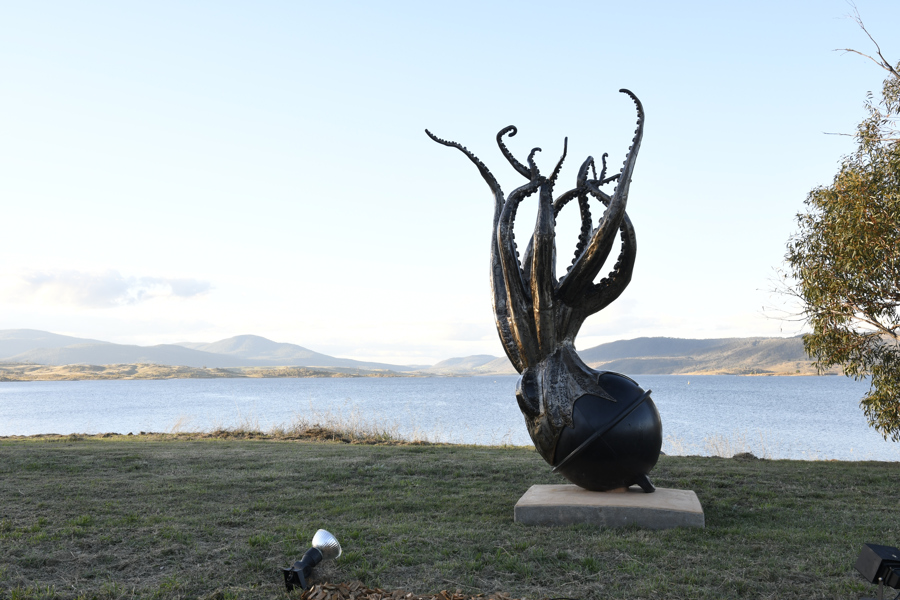
\includegraphics[width=\linewidth]{imagenes/dataset_examples/sculpture.jpg}
        \caption*{Sculpture}
    \end{subfigure}
    \caption{Ejemplos de clases en el dataset \texttt{PAINTING}}
    \label{fig:ejemplos-painting}
\end{figure}

En la figura~\ref{fig:ejemplos-painting} se han mostrado una imagen de cada una de las clases del dataset \texttt{PAINTING},
para que se pueda observar la variabilidad de las imágenes.

\subsubsection{Estructura del Dataset}
\begin{figure}[ht]
    \centering
    \begin{forest}mydirstyle
        [Dataset
            [Train (originalmente training\_set)
                [drawings
                            [image1.jpg]
                            [image2.jpg]
                            [\dots]
                    ]
                    [paintings
                            [image1.jpg]
                            [image2.jpg]
                            [\dots]
                    ]
                    [sculptures]
                    [engravings]
                    [iconography]
            ]
            [Test (originalmente validation\_set)
                [drawings]
                    [paintings]
                    [sculptures]
                    [engravings]
                    [iconography]
            ]
        ]
    \end{forest}
    \caption{Estructura de carpetas del dataset \texttt{PAINTING}}
    \label{fig:estructura-painting}
\end{figure}

Como se puede observar en la Figura~\ref{fig:estructura-painting}, las imágenes están organizadas en directorios según su categoría artística,
que en este caso corresponden a las distintas clases del dataset, previamente divididas en conjuntos de entrenamiento y prueba.

\subsubsection{Formato de los Datos}
Todas las imágenes están en formato JPEG (\texttt{.jpg}) y presentan variaciones en resolución y dimensiones.
Se han aplicado técnicas de preprocesamiento para homogenizar las características de las imágenes.

\subsubsection{Uso del Dataset}
Este dataset se ha utilizado para entrenar y evaluar modelos de clasificación de imágenes en un entorno diferente al
RPS\@.
Con este dataset, se ha comprobado el funcionamiento para evaluar los algoritmos con un dataset un poco mas complejo
que el RPS, con un par de clases más y con un número mayor de imágenes.

\subsubsection{Correcciones en la División de Datos}
Observando los tamaños de la división de los datos, y teniendo en cuenta que la divisón de los datos suele ser en train
y test, se ha decidido por renombrar las particiones de \texttt{valid} por \texttt{test} para que corresponda
correctamente con su propósito.
Y el set de validation lo he obtenido separando el set de train, normalmente haciendo una división 80\% test y 20\%
valid.

\subsubsection{Acceso al Dataset}
Inicialmente, el dataset se descargó desde Kaggle~\cite{OriginalArtImages}

Sin embargo, debido a la presencia de archivos innecesarios y algunas imágenes corruptas, se opta por una versión
limpia disponible en Kaggle~\cite{CleanedArtImages}.

\subsubsection{Licencia y Uso}
Antes de su uso, se revisaron los términos y condiciones establecidos en la página de Kaggle para asegurar el
cumplimiento con las licencias y restricciones aplicables.

\subsection{CIFAR-10}\label{subsec:cifar10}
El \textbf{CIFAR-10} es un conjunto de datos clásico de visión por computador propuesto por la Universidad de Toronto y el Canadian Institute for Advanced Research (CIFAR)~\cite{CIFAR10}.
Consta de 60\,000 imágenes en color, divididas en 10 clases equilibradas
(\emph{airplane}, \emph{automobile}, \emph{bird}, \emph{cat}, \emph{deer}, \emph{dog}, \emph{frog}, \emph{horse}, \emph{ship} y \emph{truck}).

\begin{figure}[htp]
    \centering
    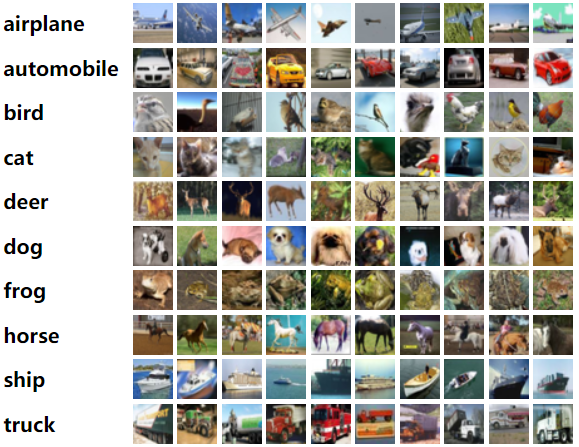
\includegraphics[width=0.7\textwidth]{imagenes/dataset_examples/cifar10-example.png}
    \caption{Ejemplos de cada clase en el dataset CIFAR-10}
    \label{fig:ejemplos-cifar10}
\end{figure}

En la figura~\ref{fig:ejemplos-cifar10} se han mostrado diez imágenes de cada una de las clases del dataset \texttt{CIFAR-10},
para que se pueda observar la variabilidad de las imágenes.

\subsubsection{Estructura del Dataset}
CIFAR-10 se distribuye en dos particiones predeterminadas:
\textbf{50.000} imágenes de entrenamiento (cinco lotes de 10.000) y \textbf{10.000} imágenes de prueba (un lote).
Al usar \texttt{torchvision.datasets.CIFAR10}, la descarga y la partición quedan gestionadas automáticamente.

\begin{figure}[ht]
    \centering
    \begin{forest}mydirstyle
        [CIFAR10
            [train: 50\,000 imgs]
            [test: 10\,000 imgs]
        ]
    \end{forest}
    \caption{Estructura lógica del dataset CIFAR-10}
    \label{fig:estructura-cifar10}
\end{figure}

\subsubsection{Formato de los Datos}
Las imágenes se almacenan comprimidas en ficheros \texttt{.bin}.
Cada imagen es RGB de 32x32 píxeles.
Al integrar el dataset con \texttt{torchvision}, se aplicaron transformaciones estándar consistentes en:
\begin{itemize}
    \item Redimensionado a 224x244 píxeles (para adaptarse a arquitecturas como MobileNet o ResNet).
    \item Conversión a tensor con \texttt{ToTensor()}.
    \item Normalización con media y desviación estándar estándar para CIFAR-10: $(0.5, 0.5, 0.5)$.
\end{itemize}

No se utilizaron pesos preentrenados ni transformaciones específicas dependientes del modelo, dado que CIFAR-10 no dispone de \textit{weights} predefinidos en \texttt{torchvision}.

\subsubsection{Uso del Dataset}
CIFAR-10 se ha empleado para comprobar el comportamiento de los algoritmos en un problema de clasificación multiclase de dificultad media-alta:
imágenes pequeñas, gran variabilidad intraclase y 10 categorías.
Esto permite evaluar la capacidad de generalización de los algoritmos meméticos en un escenario muy usado en la literatura.

\subsubsection{Licencia y Acceso}
El dataset CIFAR-10 está disponible públicamente y se distribuye bajo la licencia \emph{MIT}.
Se descarga automáticamente al ejecutar el código, sin necesidad de registro adicional.


\subsection{Comparación entre datasets}\label{subsec:comparacion-entre-datasets}
Gracias a la tabla~\ref{tab:resumen-datasets} que con las características más relevantes de los datasets utilizados,
permite entender mejor la complejidad relativa de cada conjunto y cómo pueden influir en el comportamiento de los algoritmos:

\begin{table}[htp]
    \centering
    \resizebox{\textwidth}{!}{
        \begin{tabular}{|l|c|c|c|c|}
            \hline
            \textbf{Dataset}      & \textbf{Nº Imágenes} & \textbf{Nº Clases} & \textbf{Formato} & \textbf{Tamaño Imagen} \\
            \hline
            Rock, Paper, Scissors & 2.925                & 3                  & JPG              & 300×300 px             \\
            PAINTING              & 8.576                & 5                  & JPG              & Variable               \\
            CIFAR-10              & 60.000               & 10                 & BIN              & 32×32 px               \\
            \hline
        \end{tabular}
    }
    \caption{Resumen comparativo de los datasets utilizados}
    \label{tab:resumen-datasets}
\end{table}

La selección de estos tres datasets responde a la necesidad de evaluar los algoritmos en distintos niveles de complejidad.

El dataset \textbf{Rock, Paper, Scissors} se utiliza en las primeras fases del proyecto como punto de partida,
ya que ofrece un entorno sencillo y controlado, con un número reducido de clases y una estructura equilibrada.
Esto permite desarrollar las bases del sistema y probar las primeras versiones de los algoritmos de manera más ágil y con menor coste computacional.

Posteriormente, se emplea el dataset \textbf{PAINTING} para validar el comportamiento de los algoritmos en un entorno más exigente.
Al incluir cinco categorías de arte con distintos estilos visuales, este conjunto introduce una mayor variabilidad tanto semántica como estructural,
lo que permite evaluar la robustez y capacidad de generalización de las soluciones desarrolladas.

Finalmente, se incorpora el dataset \textbf{CIFAR-10}, ampliamente utilizado en la literatura científica, para analizar el rendimiento de los algoritmos
en un entorno estandarizado y con mayor dificultad intrínseca.
Con diez clases y una alta variabilidad visual, CIFAR-10 supone un desafío adicional tanto en términos de precisión como de capacidad de generalización,
lo que permite obtener una evaluación más completa de la eficacia de los algoritmos propuestos.


\section{Diseño de los experimentos}\label{sec:diseño-de-los-experimentos}
La fase experimental se organiza en varias etapas.
Inicialmente se opta por un dataset simple (\textit{Rock, Paper, Scissors}) para validar el funcionamiento general del sistema.
Posteriormente, se realizan pruebas con datasets más exigentes.
Los experimentos se repiten utilizando diferentes porcentajes iniciales de datos (10\%, 25\%, 50\% y 75\%)
para estudiar cómo afecta la cantidad de datos seleccionados al rendimiento del modelo.

Con el fin de asegurar la consistencia entre ejecuciones experimentales, se aplican las medidas de control de reproducibilidad
descritas en el \hyperref[sec:consideraciones-de-optimizacion]{Apartado~\ref*{sec:consideraciones-de-optimizacion}}.
Esto permite comparar algoritmos en condiciones homogéneas, evitando variaciones indeseadas causadas por componentes aleatorios del entorno de ejecución.

En cada prueba, se realizan 5 ejecuciones en paralelo, cada una utilizando una semilla distinta.
Esta estrategia permite obtener resultados promedio más robustos frente a la aleatoriedad del proceso evolutivo, asegurando una mayor fiabilidad estadística.

Los apartados siguientes explican con mayor detalle el procedimiento adoptado para llevar a cabo dichas ejecuciones.


\section{Procedimiento de Ejecución y Evaluación}\label{sec:procedimiento-de-ejecucion-y-evaluacion}
Para garantizar la consistencia y objetividad en la comparación entre algoritmos, se diseñan un procedimiento experimental sistemático y replicable.
Cada ejecución se realizó bajo las mismas condiciones computacionales y utilizando los mismos parámetros base,
salvo en aquellos casos en que se deseaba estudiar una variación concreta, como los distintos porcentajes iniciales o el uso de metaheurísticas con porcentajes libres.

\subsection{Métricas de Evaluación}\label{sec:metricas-de-evaluacion}
Para evaluar el rendimiento de los modelos se utilizaron métricas estándar como \textbf{accuracy}, \textbf{precisión}, \textbf{recall} y \textbf{F1-score},
calculadas sobre el conjunto de validación tras cada evaluación.
Para una definición formal de estas métricas, véase el \hyperref[sec:metricas-evaluacion]{Apartado~\ref*{sec:metricas-evaluacion}}.

Estas métricas se calcularon utilizando las funciones de \texttt{scikit-learn}, a partir de las predicciones del modelo y las etiquetas
reales correspondientes a los subconjuntos de imágenes seleccionados por cada algoritmo.

\subsection{Evaluaciones por Ejecución}\label{sec:evaluaciones-por-ejecucion}
Se buscó un equilibrio entre la cantidad de evaluaciones y el tiempo de ejecución, permitiendo una exploración suficiente del espacio de soluciones sin comprometer la eficiencia computacional.
Por ello, cada algoritmo se configura para realizar un máximo de 100 evaluaciones por ejecución,
independientemente del tipo de algoritmo utilizado, con el fin de mantener la equidad comparativa.

Cada evaluación consiste en generar un subconjunto de datos, entrenar el modelo correspondiente (ResNet50 o MobileNetV2),
y calcular su \textit{fitness} de acuerdo con las métricas mencionadas.

El número de evaluaciones sin mejora también se monitoriza para aplicar criterios de parada anticipada,
explicados previamente en el \hyperref[sec:consideraciones-de-optimizacion]{Apartado~\ref*{sec:consideraciones-de-optimizacion}},
reduciendo así el tiempo computacional en caso de estancamiento.

\subsection{Repeticiones y Semillas}\label{sec:repeticiones-y-semillas}
Con el objetivo de obtener resultados estadísticamente significativos y reducir el efecto de la aleatoriedad,
cada configuración experimental se ejecuta 5 veces, utilizando 5 semillas distintas.
Los resultados presentados en las tablas y gráficos corresponden a la media de esas ejecuciones,
junto con medidas de dispersión cuando procede, como los boxplots.

Cabe destacar que, en el caso de los boxplots, en lugar de representar la media de las 5 ejecuciones por configuración,
se opta por incluir todos los valores individuales obtenidos con las distintas semillas.
Esta decisión permite visualizar una distribución más realista del comportamiento de cada algoritmo,
resaltando mejor la mediana, así como los valores máximos y mínimos alcanzados durante las ejecuciones.

\subsection{Tiempos de Ejecución}\label{sec:tiempos-de-ejecucion}
Cada evaluación implica entrenar un modelo desde cero, por lo que los tiempos de ejecución son considerables.
Por ejemplo, una ejecución completa con 100 evaluaciones puede tardar entre 30 minutos y 2 horas,
dependiendo del algoritmo y del modelo utilizado.

Los algoritmos más complejos, como el memético o las versiones con reinicio poblacional,
requieren un mayor tiempo de ejecución debido a las operaciones adicionales de mejora local o regeneración de población.


\section{Visualización de resultados}\label{subsec:visualizacion-de-resultados}
Para facilitar la comparación entre algoritmos, en el resto del trabajo se incluyen representaciones gráficas de los
resultados obtenidos mediante \textbf{boxplots} y \textbf{barplots}.
Ambos tipos de gráficos permiten visualizar el comportamiento global de cada algoritmo a partir de múltiples ejecuciones con distintas semillas.

\textbf{Los boxplots} (diagramas de caja) muestran la distribución estadística de los valores obtenidos.
En la Figura~\ref{fig:boxplot-explicado} se presenta un ejemplo anotado que ilustra las distintas partes de este tipo de gráfico.
La línea central de la caja representa la \textbf{mediana},
mientras que los bordes inferior y superior corresponden al \textbf{primer cuartil} (Q1) y \textbf{tercer cuartil} (Q3), respectivamente.
La diferencia entre ellos define el \textbf{rango intercuartílico} (\textit{IQR}), que contiene el 50\% central de los valores.
Las líneas que se extienden desde la caja (conocidas como \textit{bigotes}) alcanzan típicamente hasta 1.5 veces el IQR.
Los puntos que quedan fuera de ese rango se consideran \textbf{valores atípicos}, lo que permite detectar ejecuciones excepcionales.
Esta representación es especialmente útil para comparar la tendencia central, la dispersión y la estabilidad de los resultados obtenidos por los distintos algoritmos.

\begin{figure}[H]
    \centering
    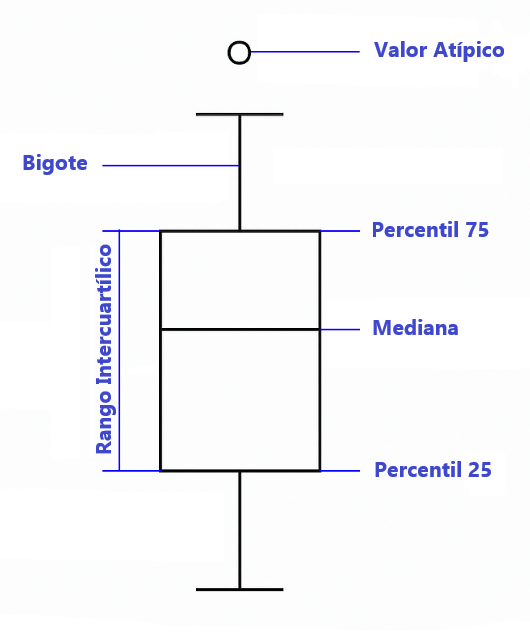
\includegraphics[width=0.45\textwidth]{imagenes/boxplot-explicado.png}
    \caption{Ejemplo de boxplot explicado.}
    \label{fig:boxplot-explicado}
\end{figure}

\textbf{Los barplots} (gráficos de barras), por su parte, se emplean para representar valores agregados como medias o proporciones,
y son útiles para observar cómo varía una métrica concreta entre distintos algoritmos, modelos o configuraciones.
Además, los barplots muestran unas barras de error que indica la desviación estándar de los valores,
lo que permite apreciar la variabilidad de los resultados obtenidos en las distintas ejecuciones.

\textbf{Los scatter plots} (diagramas de dispersión) permiten visualizar de forma conjunta la relación entre el
porcentaje inicial de datos seleccionados y el porcentaje final alcanzado tras aplicar los algoritmos.
En estos gráficos, cada punto representa una ejecución concreta, donde:

\begin{itemize}
    \item El eje \textbf{X} indica el \textbf{Porcentaje Inicial} de datos usados.
    \item El eje \textbf{Y} muestra el \textbf{Porcentaje Final} de datos seleccionados por el algoritmo tras la ejecución.
    \item El \textbf{color} y el \textbf{tamaño} de los puntos reflejan el \textbf{accuracy} alcanzado: los puntos más grandes
          y con tonos más intensos corresponden a ejecuciones con mayor precisión.
\end{itemize}

Además, cada punto se conecta mediante líneas de guía horizontales y verticales a los ejes, lo que facilita la interpretación de su posición exacta.
Estas líneas ayudan a identificar rápidamente los valores individuales en ambos ejes, mejorando la legibilidad del gráfico.

Este tipo de visualización es especialmente útil para analizar cómo los algoritmos ajustan el tamaño del subconjunto de datos en función de las condiciones iniciales,
y cómo esta selección influye en la precisión del modelo.
Permite detectar patrones como agrupamientos de soluciones o dispersiones, y observar cómo ciertas configuraciones iniciales tienden a producir mejores o peores resultados.


\section{Nomenclatura simplificada de los algoritmos}\label{subsec:nomenclatura-algoritmos}
Para facilitar la lectura de las tablas y gráficos presentados a lo largo de este trabajo,
se opta por utilizar abreviaciones consistentes para referirse a los algoritmos implementados.
Estas abreviaciones permiten condensar la información visualmente sin perder la claridad en la interpretación de los resultados.

La correspondencia entre el nombre completo de cada algoritmo y su abreviatura se muestra en la Tabla~\ref{tab:nombres-algoritmos}.

\begin{table}[htp]
    \centering
    \begin{tabular}{ll}
        \toprule
        \textbf{Nombre Completo del Algoritmo}                 & \textbf{Abreviatura} \\
        \midrule
        Aleatorio (Random Search)                              & RS                   \\
        Búsqueda Local (Local Search)                          & LS                   \\
        Búsqueda Local Libre                                   & LS-F                 \\
        Algoritmo Genético                                     & GA                   \\
        Genético con Cruce Ponderado (Weighted Crossover)      & GA-WC                \\
        Genético con Mutación Adaptativa (Adaptive Mutation)   & GA-AM                \\
        Genético con Mutación Adaptativa Libre                 & GA-AM-F              \\
        Genético con Reinicio Poblacional (Population Restart) & GA-PR                \\
        Algoritmo Memético                                     & MA                   \\
        Algoritmo Memético Libre                               & MA-F                 \\
        \bottomrule
    \end{tabular}
    \caption{Nomenclatura simplificada de los algoritmos.}
    \label{tab:nombres-algoritmos}
\end{table}

A partir de este punto, todas las tablas y gráficos del documento utilizarán estas abreviaturas para referirse a los algoritmos,
mejorando la legibilidad de los resultados y facilitando la interpretación de las comparativas entre métodos.


\section{Estructura de las Tablas de Resultados}\label{subsec:estructura-tablas}
En los siguientes capítulos, algunos resultados obtenidos a partir de los experimentos se presentan de forma tabulada para facilitar la
comprensión y el análisis comparativo entre algoritmos, modelos y configuraciones.
Estas tablas recogen las métricas de rendimiento clave obtenidas a lo largo de las distintas ejecuciones.

Las columnas principales que pueden aparecer en las tablas son las siguientes:
\begin{itemize}
    \item \textbf{Porcentaje Inicial}: Indica el porcentaje inicial de datos seleccionados por el algoritmo para cada ejecución.
          Este valor permite analizar cómo varía el rendimiento del modelo en función de la cantidad de datos utilizados.
    \item \textbf{Evaluaciones Realizadas}: Número total de evaluaciones efectuadas por el algoritmo en cada configuración.
          Generalmente, este valor se fija en 100, salvo en casos concretos como la evaluación con el 100\% del conjunto de datos.
    \item \textbf{Duración Total}: Tiempo total requerido para completar todas las evaluaciones de una configuración, expresado en formato \textit{horas:minutos:segundos}.
          Este campo ayuda a comparar la eficiencia computacional de los algoritmos.
          Se obtiene a partir de las distintas ejecuciones del algoritmo con diferentes semillas.
    \item \textbf{Duración por Evaluación}: Tiempo necesario para realizar un único entrenamiento, permitiendo evaluar la rapidez de cada modelo de forma precisa.
          Este valor se calcula dividiendo la duración total entre el número de evaluaciones realizadas.
    \item \textbf{Accuracy (Avg)}: Precisión media alcanzada, expresada en porcentaje, calculada sobre el conjunto de validación.
          Se obtiene a partir de las distintas ejecuciones del algoritmo con diferentes semillas.
    \item \textbf{Precision (Avg)}: Media de la precisión por clase (macro promedio), que refleja la proporción de verdaderos positivos entre todas las predicciones positivas para cada clase.
    \item \textbf{Recall (Avg)}: Media del \emph{recall} por clase, que indica la proporción de verdaderos positivos entre todas las instancias reales de cada clase.
    \item \textbf{F1-score (Avg)}: Media armónica entre precisión y \emph{recall}, calculada por clase y luego promediada (macro promedio).
          Es una métrica clave para problemas multiclase.
\end{itemize}

En algunas tablas, los resultados se agrupan por \textbf{modelo de red neuronal} o por \textbf{porcentaje inicial},
permitiendo comparar directamente su rendimiento bajo las mismas condiciones experimentales y facilitando el análisis del impacto de la cantidad de datos seleccionados.

Por último, aclarar que las abreviaturas de los algoritmos empleadas en las tablas corresponden a las definidas en la Tabla~\ref{subsec:nomenclatura-algoritmos},
para mejorar la legibilidad de los resultados y simplificar las comparaciones.

Las tablas están diseñadas para ofrecer una visión clara, precisa y estructurada del impacto de cada configuración experimental en el rendimiento final de los modelos.
Esta información es fundamental para evaluar la eficacia de las estrategias de reducción de datos implementadas en este trabajo.


\section{Parámetros de los Algoritmos y del Entrenamiento}\label{subsec:parametros-algoritmos}
En este apartado se describen los principales parámetros utilizados en el desarrollo de los algoritmos de
selección de instancias y en el proceso de entrenamiento de los modelos de clasificación.
La correcta configuración de estos parámetros es fundamental para asegurar un equilibrio entre la calidad de los resultados y la eficiencia computacional.

\subsection{Parámetros Generales de los Algoritmos}\label{subsec:parametros-generales-algoritmos}
\begin{itemize}
    \item \textbf{Porcentaje inicial de selección} (\texttt{initial\_percentage}): Define el porcentaje inicial de datos seleccionados para cada ejecución.
          Se han evaluado valores como 10\%, 25\%, 50\% y 75\%.
    \item \textbf{Número máximo de evaluaciones} (\texttt{max\_evaluations}): Límite de iteraciones para cada algoritmo, generalmente fijado en 100.
    \item \textbf{Número máximo de evaluaciones sin mejora} \\(\texttt{max\_evaluations\_without\_improvement}):
          Controla la parada anticipada si no se mejora el mejor resultado durante un número consecutivo de iteraciones.
    \item \textbf{Métrica de optimización} (\texttt{metric}): Métrica utilizada para calcular el fitness,
          siendo \texttt{accuracy} la más habitual, aunque también se soportan \texttt{f1-score} y otras métricas.
    \item \textbf{Modelo de red neuronal} (\texttt{model\_name}): Arquitectura utilizada para la clasificación, como \texttt{ResNet50} o \texttt{MobileNetV2}.
\end{itemize}

\subsection{Parámetros del Entrenamiento de Modelos}\label{subsec:parametros-entrenamiento-modelos}

\begin{itemize}
    \item \textbf{Tamaño del batch} (\texttt{batch\_size}): Número de imágenes procesadas simultáneamente durante el entrenamiento.
          Se fija en 32 para equilibrar tiempo y estabilidad.
    \item \textbf{Número de épocas} (\texttt{num\_epochs}): Número de veces que el modelo se entrena sobre el subconjunto seleccionado.
          Se utiliza 10 para cada evaluación.
    \item \textbf{Tasa de aprendizaje} (\texttt{learning\_rate}): Controla la magnitud de los ajustes de pesos durante el entrenamiento.
          Se establece en 0.001 para la capa final, manteniendo el resto de la red congelada.
    \item \textbf{Dispositivo de ejecución} (\texttt{device}): Determina si el entrenamiento se realiza en CPU o GPU.
          Se prioriza el uso de GPU cuando está disponible.
\end{itemize}

\subsection{Parámetros Específicos por Algoritmo}\label{subsec:parametros-especificos-algoritmos}

\textbf{Random Search:}
\begin{itemize}
    \item No utiliza parámetros adicionales, ya que la selección de instancias es completamente aleatoria.
\end{itemize}

\textbf{Búsqueda Local:}
\begin{itemize}
    \item \textbf{Tamaño del vecindario} (\texttt{neighbor\_size}): Número de imágenes modificadas en cada generación de vecino, fijado en 10.
    \item \textbf{Ajuste dinámico del tamaño del subconjunto} (\texttt{adjust\_size}): Permite variar el tamaño total de las soluciones en las versiones libres.
\end{itemize}

\textbf{Algoritmos Genéticos:}
\begin{itemize}
    \item \textbf{Tamaño de la población} (\texttt{population\_size}): Número de individuos en cada generación, generalmente 10.
    \item \textbf{Tamaño del torneo} (\texttt{tournament\_size}): Número de soluciones evaluadas para seleccionar padres en el cruce, fijado en 3.
    \item \textbf{Tasa de mutación} (\texttt{mutation\_rate}): Probabilidad de modificar aleatoriamente las soluciones, fijado en 0.1.
    \item \textbf{Ajuste dinámico del tamaño del subconjunto} (\texttt{adjust\_size}): Permite modificar el tamaño del subconjunto durante la ejecución.
\end{itemize}

\textbf{Algoritmo Memético:}
\begin{itemize}
    \item \textbf{Probabilidad de búsqueda local} (\texttt{local\_search\_probability}): Probabilidad de aplicar una búsqueda local a un individuo, fijada en 0.2.
    \item \textbf{Número de evaluaciones de búsqueda local} \\(\texttt{local\_search\_evaluations}): Máximo de evaluaciones locales por individuo, fijado en 10.
    \item \textbf{Tamaño del vecindario en búsqueda local} \\(\texttt{local\_search\_neighbor\_size}): Número de cambios permitidos en cada iteración de búsqueda local.
          Fijado en 5.
    \item \textbf{Ajuste dinámico del tamaño del subconjunto} (\texttt{adjust\_size}): Permite modificar el tamaño del subconjunto durante la ejecución.
\end{itemize}

\subsection*{}
La combinación de estos parámetros permite un control detallado del proceso de selección de instancias y del entrenamiento de los modelos,
asegurando resultados reproducibles, eficientes y de calidad.
